\documentclass[12pt,a4paper,english,twoside]{book}
\usepackage[german,main=english]{babel}
\usepackage[T1]{fontenc} 
\usepackage[latin1]{inputenc}
\usepackage{csquotes}
\usepackage{amsfonts}
\usepackage{amsmath}
\usepackage{latexsym}
\usepackage{amssymb}
\usepackage{epsfig}
\usepackage{moreverb}
\usepackage{rotating}
\usepackage{enumerate}
\usepackage{graphics, graphicx,wrapfig}
\usepackage{fancybox}
\usepackage{picinpar,varioref,floatflt}
\usepackage{ae}
\usepackage{longtable}
\usepackage[hidelinks]{hyperref}
\usepackage{textcomp}
\usepackage{float}
\usepackage{url}
\usepackage{unizhdt}
\usepackage[abbreviations, nonumberlist, shortcuts, automake]{glossaries-extra}
\makeglossaries
\newabbreviation{sc}{SC}{Smart Contract}
\newabbreviation{icom}{ICOM}{International Council of Museums}
\newabbreviation{nft}{NFT}{Non-Fungible Token}
\newabbreviation{iot}{IoT}{Internet-of-Things}
\newabbreviation{zkp}{ZKP}{Zero-Knowledge Proof}
\newabbreviation{rpc}{RPC}{Remote Procedure Call}
\newabbreviation{csg}{CSG}{Communication Systems Group}
\newabbreviation{ifi}{IfI}{Department of Informatics}
\newabbreviation{uzh}{UZH}{University of Zurich}
\newabbreviation{rest}{REST}{Representational State Transfer}
\newabbreviation{api}{API}{Application Programming Interface}
\newabbreviation{gpio}{GPIO}{General Purpose Input/Output}
\newabbreviation{http}{HTTP}{Hypertext Transfer Protocol}
\newabbreviation{abi}{ABI}{Application Binary Interface}
\newabbreviation{json}{JSON}{JavaScript Object Notation}
\newabbreviation{jwt}{JWT}{JSON Web Token}
\newabbreviation{id}{ID}{Identifier}

\newglossaryentry{wallet}{
    name={wallet},
    description={A blockchain wallet is a digital account that allows users to securely store, manage, and interact with their digital assets, such as cryptocurrencies or non-fungible tokens. It stores the private keys used to access and manage the assets on the blockchain and can be in the form of a software application or a physical device.}
}
\newglossaryentry{on-chain}{
    name={on-chain},
    description={In the blockchain context, on-chain refers to data or transactions that are recorded on the blockchain itself, rather than \gls{off-chain} or in a separate database.}
}
\newglossaryentry{off-chain}{
    name={off-chain},
    description={In the blockchain context, off-chain refers to data or transactions that are not recorded on the blockchain itself, but instead are stored or processed outside of the blockchain, such as in a separate database or through an external service.}
}


\usepackage[
    backend=biber,
    style=numeric,
    natbib=false,
    maxcitenames=2,
    minbibnames=1, maxbibnames=99, 
    url=false, 
    doi=true,
    ]{biblatex}
\addbibresource{references.bib}

\DeclareBibliographyDriver{misc}{%
    \printnames{author}%
    \newunit%
    \printfield{year}%
    \newunit%
    \printfield{title}%
    \newunit%
    \printfield{url}%
    \newunit%
    \printfield{booktitle}% used to display last-accessed for websites due to a limitation of mendeley api
    \finentry
}

%%%%%%%%%%%%%%%%%%%%%%%%%%%%%%%%%%%%%%%%%%%%%%%%%%

% Define the language of the diploma thesis
\selectlanguage{english}
%\selectlanguage{german}

\pagestyle{headings}

\begin{document}

%%%%%%%%%%%%%%%%%%%%%%%%%%%%%%%%%%%%%%%%%%%%%%%%%%

% Define the author printed on the cover page
\author{Jordi K\"uffer}
% Define the city and country of the author
\authorcity{Zurich, Switzerland}
% Define the student ID (Matrikelnummer)
\studentid{20-714-051}
% Define the title with optional subtitle
\title{Art Tracking with IoT and Blockchains}
% Define the supervisors
\supervisors{Dr. Eryk Schiller, Dr. Thomas Bocek, Prof. Dr. Burkhard Stiller}
% Define the submission date
\submissiondate{September 6th, 2023}

%%%%%%%%%%%%%%%%%%%%%%%%%%%%%%%%%%%%%%%%%%%%%%%%%%

% Make the title page
\maketitle

% Make the imprint on the back of the cover page
\makeimprint

\pagenumbering{roman}

% Include the files of the diploma thesis
%\cleardoublepage
%===============================================================================
%%%%%%%%%%%%%%%%%%%%%%%%%%%%%%%%
% Recipe to do an abstract:
%%%%%%%%%%%%%%%%%%%%%%%%%%%%%%%%
%(1) Context
%(2) Research Gap
%(3) Goals, Objectives
%(4) Methodology, how
%(5) Results

% Example:
%Abstract
%(1) In the context of energy efficiency in computer networks, a significant number of solutions ranging from protocols and functionalities to energy efficiency-oriented management applications have been proposed. 
%(2) However, the characteristics of environments to develop and validate such solutions are not as discussed as the solutions themselves. 
%(3) Considering this, this work proposes an emulation environment to develop and validate energy efficiency-oriented solutions, as well as discuss their specific characteristics. 
%(4) Thus, three functionalities of different network scopes are implemented, Adaptive Link Rate (interface level), Syncronized Coalescing (device level) and SustNMS (network level) in the Mininet emulation environment using the implemented software-defined networks paradigm on the POX controller. 
%(5) The environment is validated by comparing the energy savings achieved by these features in a topology inspired by the National Research Network (RNP).

\chapter*{Kurzfassung}
\addcontentsline{toc}{chapter}{Kurzfassung}
\selectlanguage{german}
Diese Arbeit befasst sich mit der Kombination von Internet of Things (IoT) und Blockchain-Technologien und konzentriert sich dabei auf die innovative Anwendung dieser Technologien im Bereich des Transports von Kunstwerken. Das zentrale Ziel ist die Einführung eines Systems, welches IoT und Blockchain nutzt, um die Überwachung und Verwaltung von Kunstwerken während des Transports zu verbessern.

Um dieses Ziel zu erreichen, wendet die Studie eine zweigleisige Methodik an. Zunächst wird eine umfassende Literaturrecherche durchgeführt, um ein grundlegendes Verständnis für die zugrundeliegenden Prinzipien aufzubauen. Anschließend wird ein angewandter Forschungsansatz ausgeführt, der die Entwicklung, Implementierung und Evaluierung eines Prototyps beinhaltet. Das Ergebnis dieser Forschungsarbeit ist ein funktionaler Prototyp, der den angestrebten Anwendungsfall unterstützt.

Das Ergebnis dieser Arbeit ist Artis, ein Prototyp, der den angestrebten Anwendungsfall unterstützt. Es wird jedoch festgestellt, dass der Prototyp noch weiter verfeinert werden muss, insbesondere im Hinblick auf den Schutz sensibler Daten und die Optimierung der Sensorgenauigkeit.

Der Wert dieser Arbeit liegt in der innovativen Verschmelzung von IoT- und Blockchain-Technologien, die einen neuen Weg zur Bewältigung von Herausforderungen im Bereich der Kunstwerkstransportation demonstriert. Dies legt die Grundlage für zukünftige Bemühungen, dieses Konzept zu einer produktionsreifen Lösung weiter zu entwickeln.


\chapter*{Abstract}
\addcontentsline{toc}{chapter}{Abstract}
\selectlanguage{english}
This thesis delves into the convergence of the Internet of Things (IoT) and Blockchain technologies, focusing on the innovative application of these technologies within artwork transportation. The main goal is to introduce a groundbreaking system that capitalizes on IoT and blockchain to enhance the tracking and management of artwork during transportation processes.

In pursuit of this goal, the study adopts a dual-pronged methodology. A comprehensive literature review provides a foundational understanding of the underlying principles. Subsequently, an applied research approach is employed, culminating in designing, implementing, and evaluating a prototype tailored to the intricacies of artwork transportation.

The outcome of this thesis is Artis, a real-world prototype that effectively supports the targeted artwork tracking use case. However, it is acknowledged that further strides are needed to refine the prototype, particularly in safeguarding sensitive data and optimizing sensor accuracy.

The significance of this work lies in its innovative amalgamation of IoT and blockchain technologies, presenting a novel avenue for addressing challenges in the artwork transportation domain. By demonstrating the feasibility of such a system, this thesis lays the groundwork for future endeavors to advance this concept into a production-ready solution.

%\cleardoublepage
\chapter*{Acknowledgments}
\addcontentsline{toc}{chapter}{Acknowledgments}
I am profoundly grateful for the invaluable guidance and unwavering support provided by my supervisors, Dr. Eryk Schiller, Dr. Thomas Bocek, and Dr. Bruno Rodrigues. Their profound insights, encouragement, and dedication have been instrumental in shaping the trajectory of this work.

I extend my appreciation to the entire Communication Systems Group (CSG), and Prof. Dr. Burkhard Stiller, whose collective expertise and collaborative spirit have enriched my research journey. Their vibrant exchange of ideas and constructive feedback has significantly contributed to the refinement of this study.

Finally, to my friends and family, your unwavering support has been my constant pillar of strength and has allowed me to thrive and succeed in my educational career.

\tableofcontents

\cleardoublepage
\pagenumbering{arabic}

\chapter{Introduction}
\label{chap:introduction}

%The. Introduction:
%I. The introduction of a paper aims to show the objectives, the work and give a view of the subject addressed. This should include:
%1. Contextualization of the work as a whole. Within this context can be placed the justifications or motivations for the execution of the work (must be consistent with the arguments defined in the project);
%2. An overview of the whole subject matter at work, without going into details or drawing conclusions. This is intended to give an overview of all the content addressed;
%3. Definition of the objectives to be achieved with the work (they must be by what was defined in the project). In some cases (completion work or have 40 pages of content) it is recommended to subdivide the objectives into two categories:
%The. General objective: it is normally defined objective in the project with a bit more complementary information;
%B. Specific objectives: There are several intermediate objectives that must be achieved so that when all of these are achieved, it is possible to meet the general objective.
%4. Explain how the work is organized. This is not to describe the content of the chapter as it is in the index/summary, but to say how and why the work was organized and created in the way it is. It seeks to show the reader the logical meaning of evolution and allow it to judge the best way to read the work;
%5. Explain the method of performing the work. To carry out the work, the student can use several methods of work such as research / bibliographic review, field research, experimentation (empirical or not), etc. It is important to inform about the method because it indicates the reasoning and type of work performed.

%II. Looking at the described items that should compose the introduction, it 's hard to imagine that it has less than one page;

%III. Many teachers consider that 50% of the grade of a written work is related to Introduction and Conclusion / Final Considerations.

The art trade is a diverse market with a wide range of stakeholders, including artists, collectors, auction houses, and art dealers, as well as a variety of middlemen, such as promoters, preservers, archivists, and curators, to name a few. Nevertheless, the entire art world revolves around art objects, which can also come in a large variety, from statues of different materials to canvases or even bananas nailed to walls. While museums own collections, they often display artworks from private collections or a variety thereof. Consequently, requiring trustworthy logistics partners who ensure the artwork is safely transported under optimal conditions and without damage presents an excellent opportunity for \gls{iot} sensors that can monitor temperature, humidity, vibrations, and other environmental factors. Additionally, blockchain technology can be leveraged to ensure the correctness of the transportation process for all stakeholders and, in combination with art trading, to ensure and document the transfer of ownership virtually and physically, thus bringing a degree of standardization to a largely unregulated and opaque market \cite{certify}.

% Why mapping physical artwork as NFTs is good? bad? Although having challenges associated with the "unique" identification of artwork, does it still present benefits? For example, tracking/tracing, reporting transport conditions? Higher transparency between museums by knowing "who did what at some point in time with a given artwork"? 

% Has someone done something similar? Do these projects provide a prototype (even if it is minimal) tested in real world? Open-source? This helps to highlight your contributions!

\section{CERTIFY Project}
\label{sec:certify}
CERTIFY is a multi-partner research project \cite{certify}, dedicated to achieving a high level of security by developing a novel framework to manage security throughout the lifecycle of \gls{iot} devices. The project is scheduled to run from 1st October 2022 for 36 months and involves 13 partners from eight European countries. The \gls{csg} of the \gls{ifi} at \gls{uzh} is part of CERTIFY and focusing on designing and developing a blockchain-based sharing infrastructure of security information, an Over-The-Air Patch Infrastructure and the pilot for tracking and monitoring of artworks. This thesis is part of the contributions by \gls{csg} to the pilot for tracking and monitoring of artworks.

\section{Motivation}
Artwork transportation has proven to be a logistical challenge in many ways \cite{artintransit}. Complying with regulatory laws of both the departure and destination country, taking out insurance on the artworks, using packaging that lowers the risk of damage, and many more. Recording all relevant transactions typically involves administrative paperwork and trust among the many parties involved \cite{artintransit}.

The \gls{iot} has revolutionized how we interact with technology and data, allowing us to connect devices, sensors, and networks seamlessly. At the same time, blockchain technology has emerged as a powerful tool for securely managing data and transactions in a decentralized, tamper-proof way. Combined, these technologies offer exciting possibilities for creating new forms of digital art that are both secure and transparent.

\gls{iot} devices, such as sensors, can record data that can be used to monitor the environment around an artwork. By using blockchain technology to manage and store this data securely, stakeholders can ensure the integrity of artwork even in a trustless environment. The blockchain ledger can additionally improve documentation of ownership and custody by indefinitely storing transactions on the chain.

In this context, the thesis proposes a system for artwork tracking in combination with hardware and software deployed to provide automatic monitoring and management of artwork in a transportation scenario.

\section{Description of Work}
The work involves creating a secure and transparent system for tracking and monitoring the movement of a unique item, represented by a \gls{nft} \cite{nftminter}, using a combination of blockchain technology and \gls{iot} devices. The goal is to develop a system for monitoring and logging some environmental parameters, such as temperature and humidity, while transporting artwork. The system should be able to define alert thresholds for these parameters and notify the artwork sender, carrier, and recipient of any anomalies. The \gls{nft} is registered in a \gls{sc} by the item owner or holder and contains relevant information and regulations, such as ObjectID \cite{objectid}, as required by the \gls{icom}.

The \gls{iot} Board Administrator sets the board to its initial state, ready to receive data from the sensors. A private and public key profile is generated and stored on the device, ensuring the private key remains confidential and cannot be leaked. The public key is registered on the blockchain and is associated with the \gls{nft} by the owner. This profile can update the state of the \gls{nft} by issuing transactions signed with the private key to the smart contract. This allows the \gls{nft} to be updated with events such as "pick up at origin" and "delivery at destination," which are logged with relevant timestamps. 
Multi-approval operations certify changes in responsibilities between different actors, such as when the Sender transfers responsibility for the artwork to the Carrier. This helps to ensure the secure and transparent transfer of custody of the item. 

Finally, with the transfer of custody, the behavior of the sensor is set from standby mode to constant monitoring mode, allowing for real-time tracking and monitoring of the item as it moves from one location to another. The system provides a secure and transparent way to track and monitor unique items' movement while ensuring their authenticity and ownership.

\subsection{Thesis Goals}
\label{sec:thesis_goals}
\begin{itemize}[font=\textbf, align=left]
    \item[Research:] The research report should include a review of the relevant literature concerning the technologies used and include existing solutions for blockchain-based artwork tracking.
    \item[Design on Solution Architecture:] The report should include detailed specifications and requirements for the system, including backend and frontend.
    \item[Solution Prototyping:] This goal covers the implementation of a prototype of the artwork tracking system. This involves working with \gls{iot} devices, sensors, and other suitable technologies. The prototype should be functional and demonstrate the key features of the system.
    \item[Evaluation:] The system evaluation involves testing the prototype in a (simulated) real-world artwork transportation scenario. The evaluation report includes an analysis of the system's performance and an assessment of its real-world usability.
\end{itemize}

\section{Methodology} % structure heavily inspired from Enforcing Privacy in a Smart Home Environment via Pi-hole Integration is this ok?
The methodology adopted in this thesis is strategically designed to comprehensively address the objectives outlined in Section \ref{sec:thesis_goals}. This approach can be categorized into two primary phases: a literature review phase and an applied research phase.

\textbf{Literature review phase:} This involves conducting a literature review to gather essential knowledge about fundamental concepts and related work in artwork tracking and blockchain and \gls{iot}. This review provides an overview of related work on tracking solutions, summarized in Table \ref{tab:related_work}. The knowledge gained will serve as a basis for the design and development of the proposed system.

\textbf{Applied research phase:} The applied research phase is composed of creating and evaluating a prototype for the proposed system. It includes the design, implementation, and evaluation described below.

\begin{itemize}[font=\itshape, align=left, itemindent=0.5cm]
    \item[Design:] The system architecture design is based on a simplified artwork tracking scenario. The prototype is required to support this scenario concerning the goals defined in Section \ref{sec:thesis_goals}. The architecture includes all necessary components and interactions to support the use case. This phase delivers a documentation of this design presented in Chapter \ref{chap:architecture_design}.
    \item[Implementation:] The output of the previous phase needs to be implemented as a prototype system. The implementation process and details regarding the implementation of features are reported in Chapter \ref{chap:implementation}. 
    \item[Evaluation:] In the final phase, the delivered prototype of the implementation phase is evaluated. The evaluation includes a cost and performance analysis outlined in Section \ref{sec:cost_and_performance}, a security analysis in Section \ref{sec:security_analysis}, and a test run in a simulated artwork tracking scenario in Section \ref{sec:field_test}. The results are discussed in Section \ref{sec:eval_discussion}.
\end{itemize}


\section{Thesis Outline}
Chapter \ref{chap:introduction} has provided introductory and motivational information. Chapter \ref{chap:technologies} gives a high-level overview of the theoretical background of the thesis. In Chapter \ref{chap:related_work}, we discuss existing papers on the topic and elaborate on the current state-of-the-art regarding artwork tracking. This information is built upon in Chapter \ref{chap:architecture_design} when we present the architecture and design of our solution in detail. The implementational aspects of the solution are presented in Chapter \ref{chap:implementation}. The implemented system is then evaluated in Chapter \ref{chap:evaluation}, and a summary and conclusions are given in Chapter \ref{chap:summary}. Furthermore, it addresses the potential for future work and suggests opportunities for improvement of the proposed system.


\chapter{Fundamentals}
\label{chap:technologies}
This chapter aims to introduce valuable background knowledge of the fundamentals built upon in this thesis.

\section{Internet of Things}
\gls{iot} technology does not have a single unique definition. However, \textcite{iot} defines the term Internet of Things as follows:
\begin{quote}
    "An open and comprehensive network of intelligent objects that have the capacity to auto-organize, share information, data, and resources, reacting and acting in face of situations and changes in the environment"
\end{quote}
While the internet in the traditional sense is about the data created by people, \gls{iot} is about data created by things. A practical example of this would be a smart heating system for a vacation home. Such a system is able to record and store data about environmental parameters such as temperature or humidity and make this data accessible in real-time on a smartphone through the internet. It is also possible to interact with this system through your phone. For example, raising the temperature of a winter vacation home the night before arrival would be possible. This thesis aims to utilize an \gls{iot} device capable of recording and storing environmental parameters to monitor an artwork in transit.

\section{Blockchain}
Blockchain technology has long been an evolution and promising advancement in distributed and decentralized systems. It describes a ledger that can be either distributed (permissioned) or decentralized (permissionless), tamper-evident, tamper-resistant and usually without a central authority. This technology allows a community of users to record transactions that cannot be changed once published \parencite{blockchainoverview}.

These properties can reduce the importance of trust among single parties, as the consensus of the whole network is necessary for a transaction to be published. This is why blockchain has been able to digitize processes that previously required trust in a central authority. The most prominent are cryptocurrencies like Bitcoin and Ethereum \cite{bitcoin, ethereum}.

\subsection{Smart Contracts}
Some blockchains can be extended and leveraged by smart contracts, essentially collections of code and data deployed on the blockchain network using cryptographically signed transactions. Nodes within the blockchain network execute the smart contract, and the results of execution are recorded on the blockchain. Users can create transactions that send data to public functions offered by a smart contract. The smart contract then executes the appropriate method to perform a service. Since the code is on the blockchain, it is tamper-evident and resistant, making it a trusted third party. Smart contracts can perform various functions such as calculations, storing information, exposing properties, and automatically sending funds to other accounts \parencite{blockchainoverview}.

\subsubsection{Non-Fungible Token}
An example of a smart contract standard would be the ERC-721 for \glspl{nft} on the Ethereum network~\cite{erc721}. \glspl{nft} are digital assets stored on a blockchain and represent a unique item or asset, such as a piece of artwork. 

\section{Tracking and Tracing}
Tracking and tracing of logistic networks is considered an important issue \cite{trackingtracing}. In this context, tracking refers to collecting and managing information about the current location and status of a product or delivery item \cite{trackingtracing}. Tracing on the other hand looks back in time and refers to the storing and retaining of a product or item's history \cite{practicetrackingtracing}.


\chapter{Related Work}
In this chapter, we provide an overview of the existing literature related to art tracking with IoT and blockchains, highlighting previous research, methods, and findings related to the research question. Lastly, we also provide an overview of the state of the art in this field.

\section{Blockchain Technology}
Blockchain technology has been proposed as a promising solution to the challenges faced in the creative industry, such as issues related to the monetization of intellectual property but also the provenance and authenticity of creative work. \cite{creativeindustry} Especially technologies like smart contracts and \glspl{nft} have shown the potential of blockchain technology to revolutionize the art market by enabling greater transparency, accountability, and traceability. 

\section{NFTs in the Art World}
 \glspl{nft} have gained significant attention in the art world in recent years, with several high-profile sales of \gls{nft}-based artworks. \textcite{nftopportunities} has shown the benefits of \glspl{nft} protecting digital assets \textcite{creativeindustry} has suggested the application of \glspl{nft} beyond digital art, proposing to physically tag an \gls{iot} device to an artwork or sculpture. This could be used to transfer and track ownership while also potentially reducing intermediaries. \textcite{artchain} for example, developed a blockchain-based trading system for artworks. And \textcite{nftminter} has proposed a \gls{nft} Minter for a blockchain-based artwork trading system. Another related study by \textcite{zkdet} proposes a traceable and privacy-preserving data exchange scheme based on \gls{nft} and \gls{zkp}.

\section{Existing Art Tracking Systems Using IoT and Blockchain}
The combination of these two technologies in industrial systems and supply chains has been a "hot trend" in recent years. \cite{industryiot} Several companies and research groups are exploring the use of IoT and blockchains for art tracking and management.

For example, Artory \cite{artory} is tokenizing physical artworks to create a secure record of art pieces' provenance and ownership. \textcite{artrentalblockchain} developed an artwork rental system based on blockchain technology that is intended to facilitate the process of lending artwork collections. Another company that is incorporating \gls{iot} and blockchain technology is Everledger \cite{everledger}. Although they have been focused on other assets than artwork they also have discovered use cases that involve artwork tracking and authentication. Authena \cite{authena} is a swiss based company that is trying to protect the authenticity and traceability of physical assets. A study by \textcite{pactart} developed an \gls{iot} architecture called PACT-ART that employs advanced computing techniques like data mining and business process intelligence to predict a future state of the process and point out any possible violation from it.





\chapter{Architecture and Design}
This chapter aims to provide a high-level overview of the architecture of the system while also going into detail about its components and actors.




\chapter{Evaluation}
\label{chap:evaluation}
In this chapter, we evaluate different aspects of the developed system. Section \ref{sec:cost_and_performance} shows a cost and a performance analysis of the developed \gls{sc}. Section \ref{sec:field_test} concludes the analyses with a field test of a simulated artwork transportation scenario. Finally, this chapter is concluded with a discussion in Section \ref{sec:eval_discussion} To evaluate the performance of the system we also recorded the response time of each request. This can give an indicator

\section{Cost and Performance Analysis}
\label{sec:cost_and_performance}
The primary cost factor of the artis-system is the \gls{sc}. Each execution of a function that mutates the state of the \gls{sc} costs a certain amount of gas which in turn has a price in Ether. The cost for a transaction thus is calculated as follows:
$$
transaction\ fee = gas \times gas\ price
$$
To analyze the execution costs of the \textit{safeMint} and \textit{updateArtworkData} contract functions, we executed the corresponding requests of the developed \gls{api} multiple times $(n = 10)$ for each input variety. This analysis was conducted on the sepolia testnet and the resulting transactions were inspected on the Etherscan block explorer. The transactions were submitted with a relatively high gas price (30 Gwei) to make the transactions attractive for validators \cite{ethergas}. During this analysis, we observed that the gas used for a specific function depends on the input parameters but does not vary if the input parameters are the same. To analyze the performance, we also recorded the processing time of each request. This time can be an indicator of the performance but depends on the state of the blockchain and likely differs on the mainnet.

To get a sense of how gas translates into fees, we used the average gas price of the past month for the Ethereum mainnet (28 Gwei, 07.08.23 - 08.08.23) \cite{gaspriceaverageethereum} and the current value of Ether in \gls{chf} (1625.20 CHF = 1 ETH, 09.08.23) \cite{coinmarketcap}. Because the contract can also be deployed on other blockchains that use the \gls{evm}, we decided to include the cost on the polygon network. Except the contract has not been deployed to the Polygon network, and the same amount of gas was used for these calculations. The average gas price of the past month (173 Gwei \cite{gaspriceaveragepolygon}, 07.08.23 - 08.08.23) was multiplied by the gas and converted into \gls{chf} by using the current price for MATIC (0.60 CHF = 1 MATIC, 09.08.23) \cite{coinmarketcap}. The results were rounded to four decimal points for the tokens and two decimal points for \gls{chf}.

\begin{figure}[ht]
    \begin{subfigure}{0.49\textwidth}
        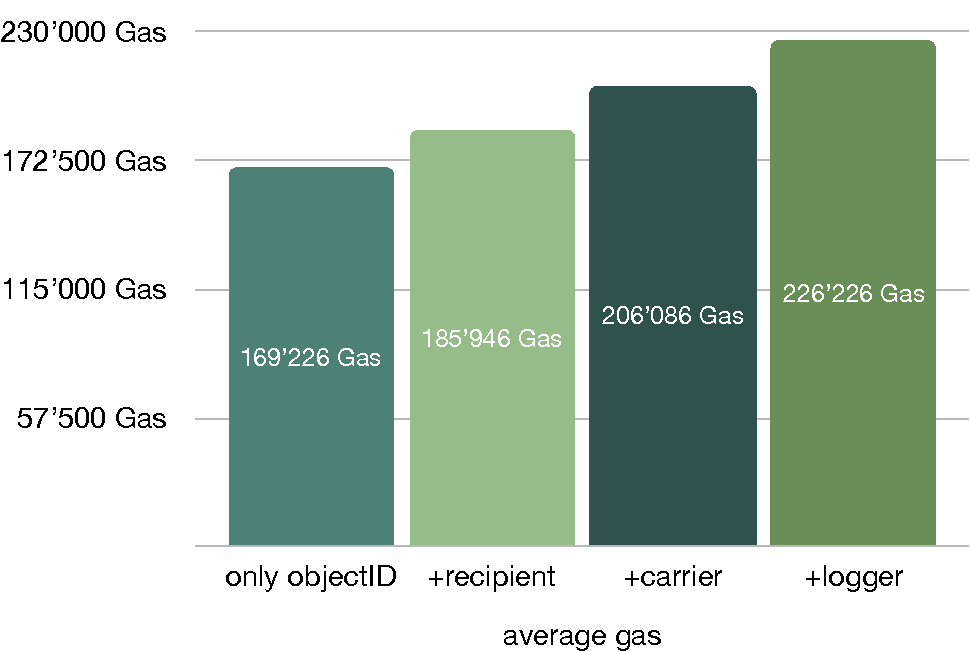
\includegraphics[width=\textwidth]{diagrams/safeMint_gas_eval.pdf}
        \caption{Transaction gas usage}
        \label{fig:safemint_tx_cost}
    \end{subfigure}
    \hfill
    \begin{subfigure}{0.49\textwidth}
        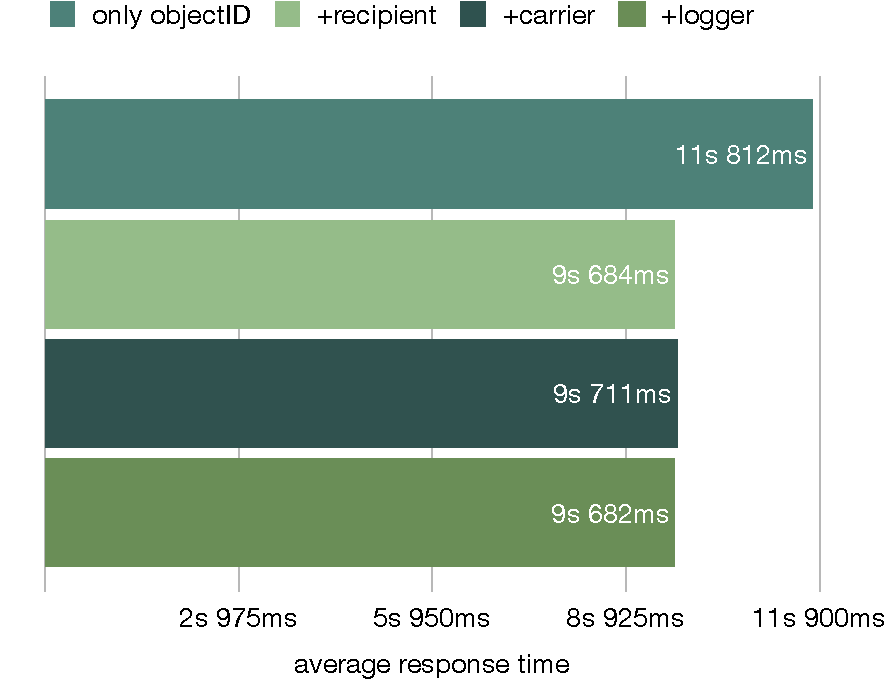
\includegraphics[width=\textwidth]{diagrams/safeMint_request_time_eval.pdf}
        \caption{Request speed in seconds}
        \label{fig:safemint_tx_speed}
    \end{subfigure}
    \caption{safeMint analysis}
    \label{fig:safemint_analysis}
\end{figure}

\subsection*{safeMint}
Figure \ref{fig:safemint_tx_cost} shows the average gas the safeMint function consumes for various input parameters. Each bar shows the average of 10 function executions. The very left bar shows the average gas used if only the objectID of the artwork is added during minting. The second bar shows the gas consumed if the objectID and the recipient address are provided during minting. This pattern remains the same for the last two bars. The analysis shows that the more parameters are provided, the more gas it consumes. Table \ref{tab:safemint_tx_fees} shows the transaction fees in the corresponding native token and converted into \gls{chf} as outlined above. 

\begin{table}[h]
\begin{adjustbox}{width=1\textwidth}
\begin{tabular}{cllll}
\multicolumn{1}{l}{}                                                           & \textbf{only objectID} & \textbf{+recipient} & \textbf{+carrier} & \textbf{+logger} \\ \hline 
\textbf{\begin{tabular}[c]{@{}c@{}}transaction fee\\ ETH (MATIC)\end{tabular}} & 0.0048 (0.0293)        & 0.0053 (0.0322)     & 0.0059 (0.0357)   & 0.0064 (0.0392)  \\ \hline
\textbf{\begin{tabular}[c]{@{}c@{}}in CHF \\ Ethereum (Polygon)\end{tabular}}  & 7.83 (0.02)            & 8.61 (0.02)         & 9.54 (0.02)       & 10.47 (0.02)    
\end{tabular}
\end{adjustbox}
\caption{Estimated transaction fees safeMint}
\label{tab:safemint_tx_fees}
\end{table}

The response time of the \gls{api} calls are mostly below 10s. We could not observe a large difference in the different input parameters. The chart in Figure \ref{fig:safemint_tx_speed} shows the average response time in seconds. The maximum response time recorded was 33s on the fifth call with only the objectID submitted, and the minimum was 3s with the objectID and recipient address submitted. This shows that this metric can fluctuate heavily depending on the state of the network.

\begin{figure}[ht]
    \begin{subfigure}{0.49\textwidth}
        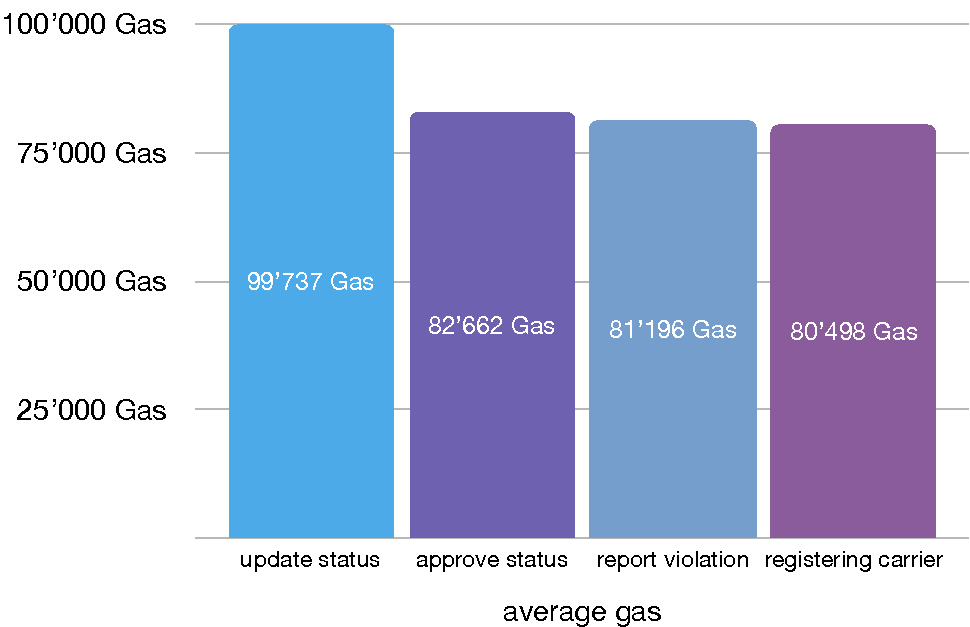
\includegraphics[width=\textwidth]{diagrams/updateArtworkData_gas_eval.pdf}
        \caption{Transaction gas usage}
        \label{fig:updateArtworkData_tx_cost}
    \end{subfigure}
    \hfill
    \begin{subfigure}{0.49\textwidth}
        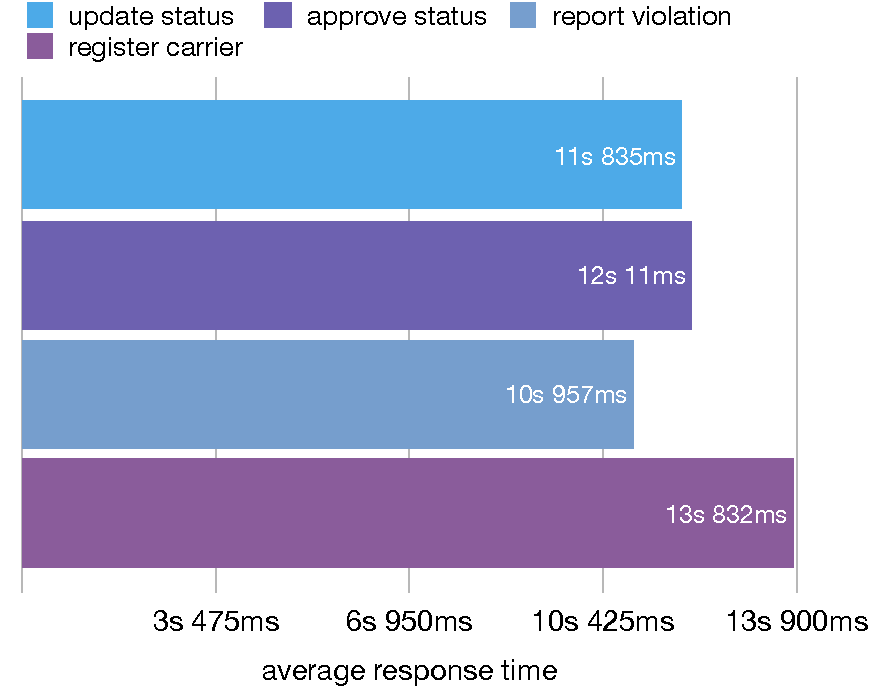
\includegraphics[width=\textwidth]{diagrams/updateArtworkData_request_time_eval.pdf}
        \caption{Request speed in seconds}
        \label{fig:updateArtworkData_tx_speed}
    \end{subfigure}
    \caption{updateArtworkData analysis}
    \label{fig:updateArtworkData_analysis}
\end{figure}

\subsection*{updateArtworkData}
Similarly, we also analyzed the updateArtworkData function. The bar on the very left of Figure \ref{fig:updateArtworkData_tx_cost} shows the average gas consumed by the function when updating the requested status. Approving the status as a different actor shows an average gas consumption of 82'662. The last two bars show the gas amount for reporting a violation from the logger and registering a carrier.

The cost of these transactions was estimated similarly to with the safeMint function (Table \ref{tab:updateArtworkData_tx_fees}). The results show that updating an artwork \gls{nft} is much less costly than minting it. 

\begin{table}[h]
\begin{adjustbox}{width=1\textwidth}
\begin{tabular}{cllll}
\multicolumn{1}{l}{}                                                           & \textbf{update status} & \textbf{approve status} & \textbf{report violation} & \textbf{register carrier} \\ \hline 
\textbf{\begin{tabular}[c]{@{}c@{}}transaction fee\\ ETH (MATIC)\end{tabular}} & 0.0028 (0.0173)        & 0.0024 (0.0143)     & 0.0023 (0.0141)   & 0.0023 (0.014)  \\ \hline
\textbf{\begin{tabular}[c]{@{}c@{}}in CHF \\ Ethereum (Polygon)\end{tabular}}  & 4.62 (0.01)            & 3.83 (0.01)         & 3.76 (0.01)       & 3.73 (0.01)    
\end{tabular}
\end{adjustbox}
\caption{Estimated transaction fees updateArtworkData}
\label{tab:updateArtworkData_tx_fees}
\end{table}

The average response time of updating an \gls{nft} varies depending on the input parameters. The request that was fulfilled the fasted approved a status change in around three Seconds. Interestingly, the longest response time of over 35 seconds was recorded on the same type of request.


\subsection*{Non-Mutating Functions}
The GET endpoints exposed by the \gls{api} target several functions that do not mutate the state of the \gls{sc}. These functions do not cost gas, and their execution time is much less (usually < 1 Second). Additionally, the artis-server adds a caching layer to these function calls, which generally reduces the response time of repeated calls to a few milliseconds.

\section{Security Analysis}
\label{sec:security_analysis}
Since the system is intended to be used by different actors in a trust-less environment a security analysis is vital for evaluating the prototype. The following section discusses the different attack surfaces and evaluates the security risk.

\subsection{Threat Scenarios}
% You can improve the analysis here by considering those aspects in terms of CIA (Confidentiality, Integrity, and Availability). 
% Even a small table with risk assessment 
\subsubsection{Compromised Logger}
The logging device is important to the system, and a compromised device would lead to a compromised system altogether. We consider three different attack scenarios when it comes to the logger.
\subsubsection{Software Exploitation}
Currently, the device itself is not secured in any way. Any malicious actor could connect to the logger device and alter its software. This could include changing the violation thresholds, stopping the logging script, manipulating the local database of the readings, and more. The current system is not protected against this threat, and thus, the security risk is high.
\subsubsection{Hardware Exploitation}
The recordings can also be influenced externally by exploiting the hardware components. By gaining access to the logger device, a malicious actor could influence the environmental parameters in a minimal perimeter around the sensor and falsify the readings. This could result in violations even if the artwork itself was not affected or could prevent violations even if the artwork was affected. The current system is not protected against this threat, and the security risk is high.
\subsubsection{Compromised Credentials}
The system only allows registered actors to change the \gls{nft}. This is also true for the logger device, which authenticates the system by signing a challenge message with a private key. If the private key is leaked, a malicious actor could report violations even if none occurred. Currently, the private key is stored in an environment variable on the software. An attacker could easily retrieve the value of the private key by connecting to the logger. This indicates a high-security risk for this threat.

\subsection{Compromised Smart Contract}
A malicious actor could influence the state of the \gls{sc} by accessing it directly. The attacker would have to identify flaws in the contract code and find an exploit to manipulate artwork data. We estimate the security risk of finding a flaw in the code to be medium, as the contract was tested during development, and basic code-checking tools could not identify a vulnerability. The \gls{sc} only accepts transactions issued by the system's admin. If the admin credentials are leaked, the attacker would have unlimited access to the \gls{sc}. In the current system, the admin's private key is only stored on the artis-server. The server is deployed as a Google Cloud-run service, and the Google secret manager supplies the private key. The security risk for this threat scenario is estimated to be low because the secret manager is an industry-standard solution for managing sensitive data.

\subsection{Disclosure of Data}
The data stored on the \gls{sc} could be sensitive depending on the use case. The \gls{sc} prevents unauthorized users from reading data. However, the transactions submitted to update data can contain sensitive information. This information can be read by anyone that has access to the \gls{sc} address, admin address, or any of the actors' addresses. Because these addresses are not considered secrets, the system must disclose all data to the public. This could introduce a high-security risk for certain use cases.

\section{Field Test}
\label{sec:field_test}
Because the isolated analyses performed above do not indicate how the system would perform during an artwork transportation scenario, we used the system on a simulated transportation scenario.

\begin{figure}[ht]
    \centering
    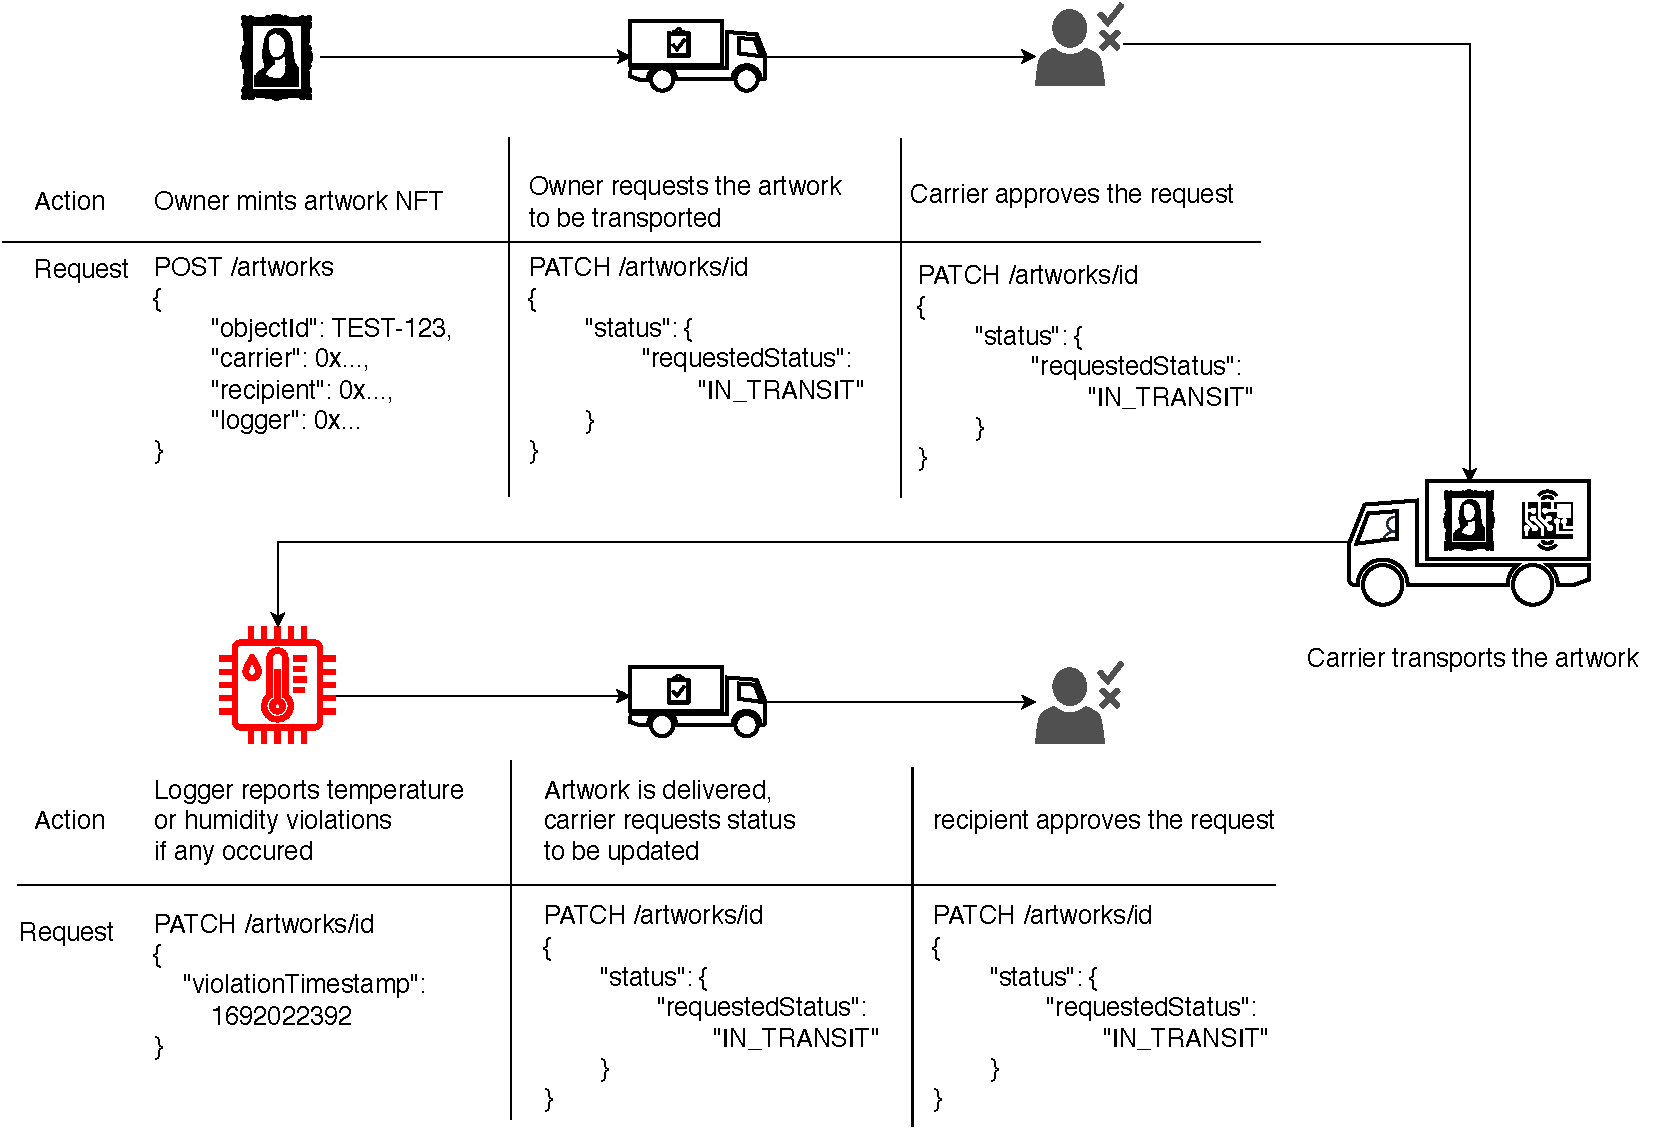
\includegraphics[width=0.9\textwidth]{diagrams/evaluation_scenario_v2.drawio.pdf}
    \caption{Field test scenario}
    \label{fig:eval_scenario}
\end{figure}

The steps of the simulated scenario are visualized in Figure \ref{fig:eval_scenario} and described in more detail below.

\begin{enumerate}
    \item Creates a new artwork \gls{nft} and registers the corresponding roles using the artis-frontend.
    \item Request the status of the artwork to be changed to \textit{IN\_TRANSIT} from the sender account
    \item Approve this request from the carrier account
    \item Enable the logger by starting the \textit{logging\_script} and the \textit{violation\_script} with the thresholds of 25 degrees Celcius and 70\% humidity.
    \item Take the logging device and transport it from the point of departure to the destination
    \item During the transportation, simulate a violation by wrapping a hand around the sensor to increase the temperature.
    \item Upon arrival, request the status of the artwork to be changed to \textit{DELIVERED} from the carrier account
    \item Approve this request from the recipient account
\end{enumerate}

\begin{figure}[ht]
    \begin{subfigure}{0.5\textwidth}
        \centering
        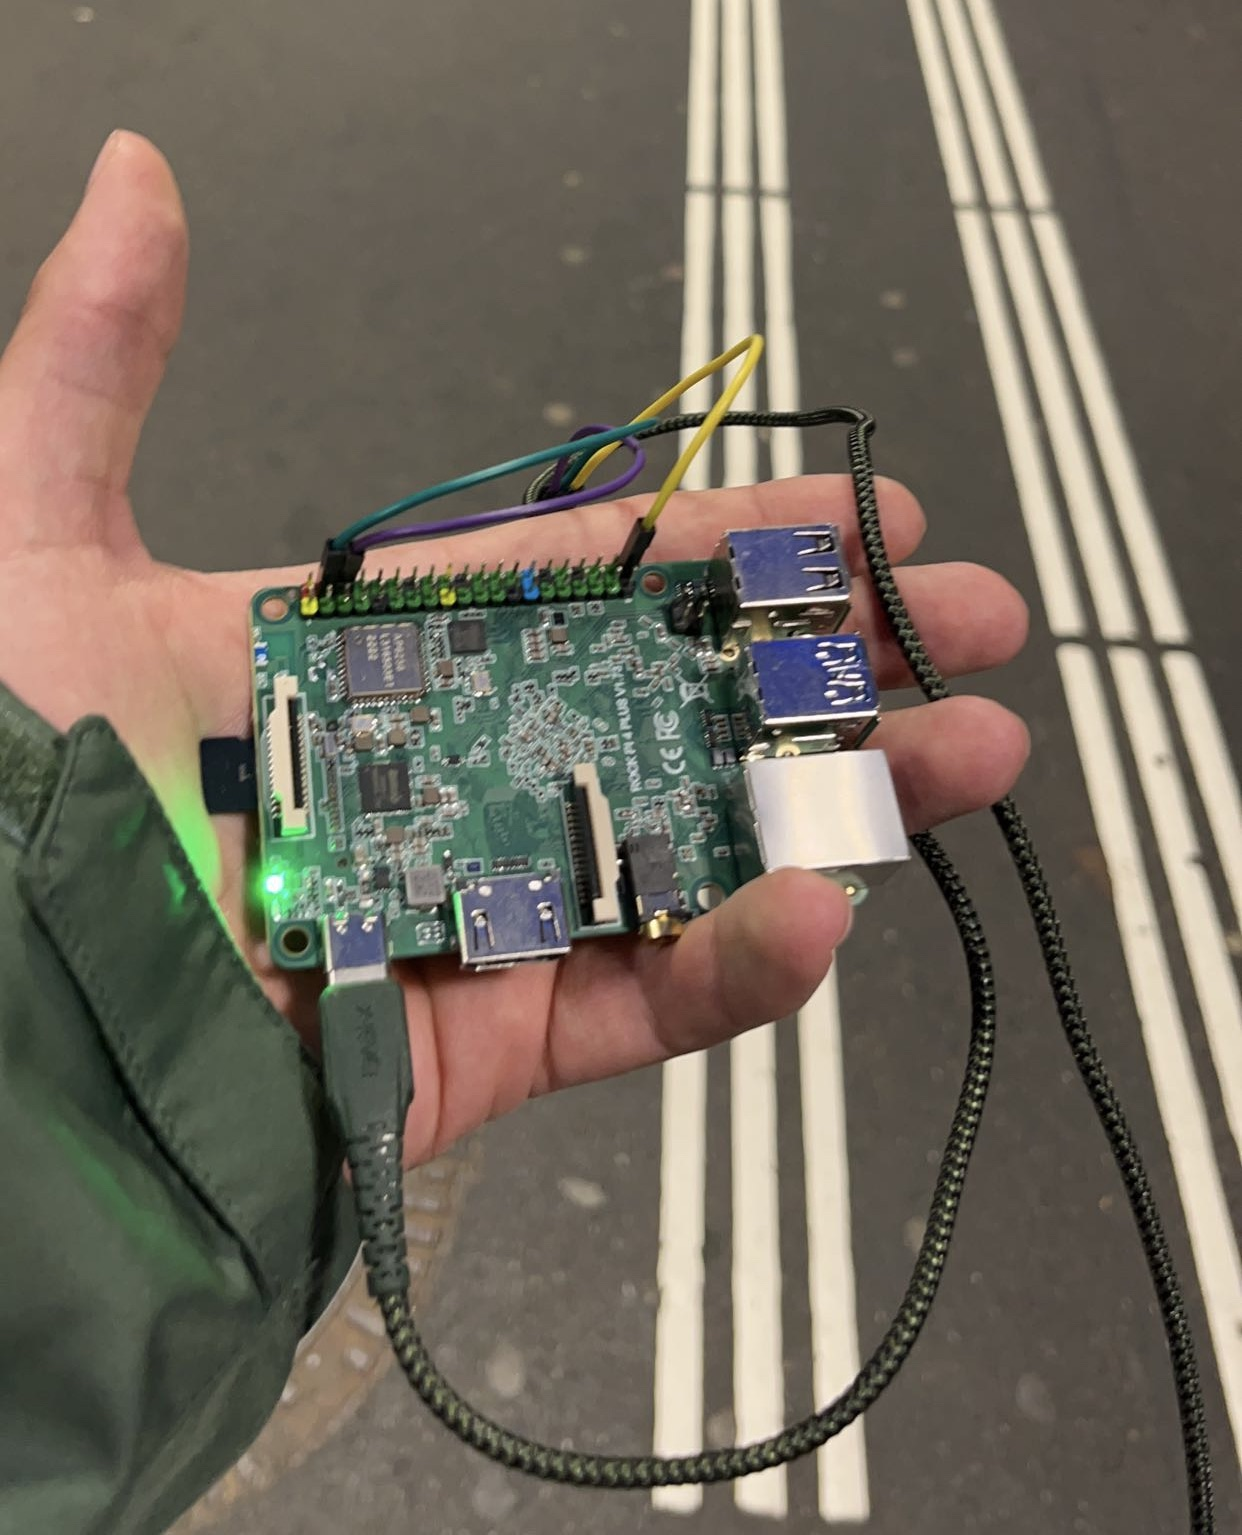
\includegraphics[height=0.25\textheight]{resources/field_test.jpeg}
        \caption{Simulating artwork transportation scenario}
        \label{fig:sensor_transport}
    \end{subfigure}
    \hfill
    \begin{subfigure}{0.5\textwidth}
        \centering 
        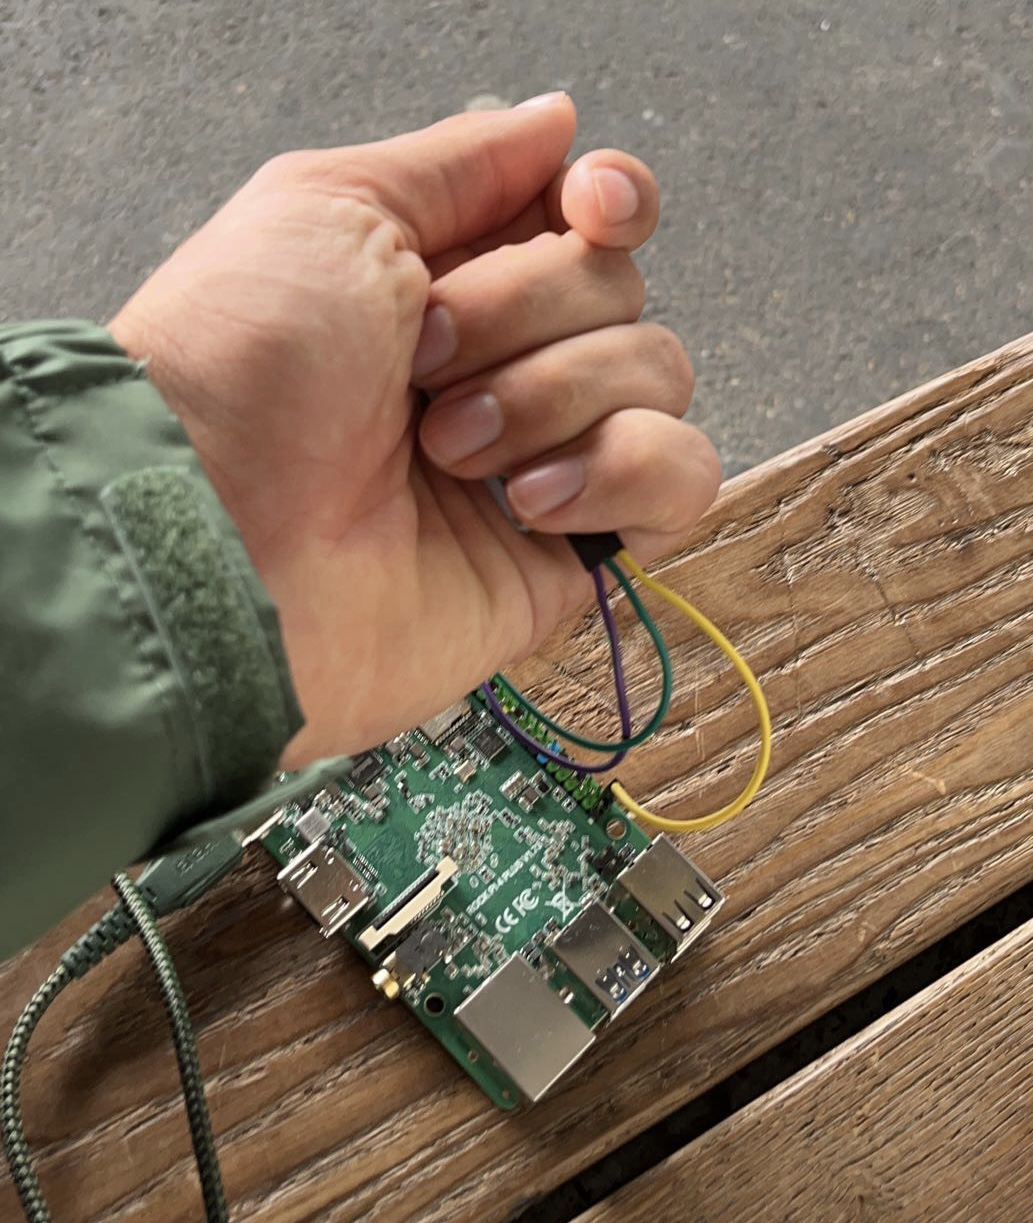
\includegraphics[height=0.25\textheight]{resources/cover_sensor.jpeg}
        \caption{Simulating temperature violation}
        \label{fig:covering_sensor}
    \end{subfigure}
    \caption{System Field Test}
    \label{fig:field_test}
\end{figure}

The field test involves a minimum of five requests to the \gls{api}. If any violations occur, this number is increased accordingly. We also simulated a temperature violation by covering the sensor with our hand (Figure \ref{fig:covering_sensor}) to include a violation in the test. The test was performed on the go, traveling by train and using a power bank to power the device and a hotspot from a cellular phone to connect to the internet. During the test, we recorded different metrics now used for evaluation. The most important metrics include a cost analysis of the field test and an evaluation of the performance of the logger.

\subsection{Cost}
During our field test, nine transactions were issued by the \gls{api}. The cost analysis also includes deploying the \gls{sc} and minting the \gls{nft}. However, this would be a one-time cost, and its significance will shrink with the number of transportation. Table \ref{tab:field_test_tx_fees} gives an overview of the transactions and estimated costs. The costs are estimated in the same manner as in Section \ref{sec:cost_and_performance}. However, the transactions were not issued with a fixed gas price, but each transaction was estimated based on the network at the time. 

The total cost of the field test mainly consists of the contract deployment. This transaction accounts for over 78\% of the total gas consumption and thus also accounts for the greatest cost factor. The variable part included in another similar transportation scenario of the same artwork amounts to around 25.85 \gls{chf} on the Ethereum network or around 0.05 \gls{chf} on the Polygon network.

\begin{table}[ht]
\centering
\begin{tabular}{lcc}
\multicolumn{1}{c}{\textbf{Transaction}} & \multicolumn{1}{l}{\textbf{Count}} & \multicolumn{1}{c}{\textbf{Total Cost on Ethereum (Polygon)}} \\ \hline
Contract deployment                      & one time                           & 143.79 (0.33)          \\
mint NFT                                 & one time                           & 12.05 (0.03)           \\
update status                            & 2                                  & 9.26 (0.02)            \\
approve status                           & 2                                  & 7.68 (0.02)            \\
report violation                         & 3                                  & 8.91 (0.03)            \\ \hline
\textbf{Total}                           & \textbf{9}                         & \textbf{181.69 (0.43)} \\
\hline
\end{tabular}
\caption{Transaction fees field test}
\label{tab:field_test_tx_fees}
\end{table}
\vspace{-0.5cm}
\subsection{Logger Reliability}
The field test lasted around 52 minutes. During the transportation, the logger stored every sensor reading in a local database. Figure \ref{fig:field_test_sensor_readings} illustrates the intervals of the sensor readings. Each line indicates a successful reading by the sensor; the red lines represent a violation. The maximum time between two readings was 9 minutes and 36 seconds. The shortest interval was less than a second. For this prototype, we did not test other metrics such as accuracy or range.

\begin{figure}[ht]
    \centering
    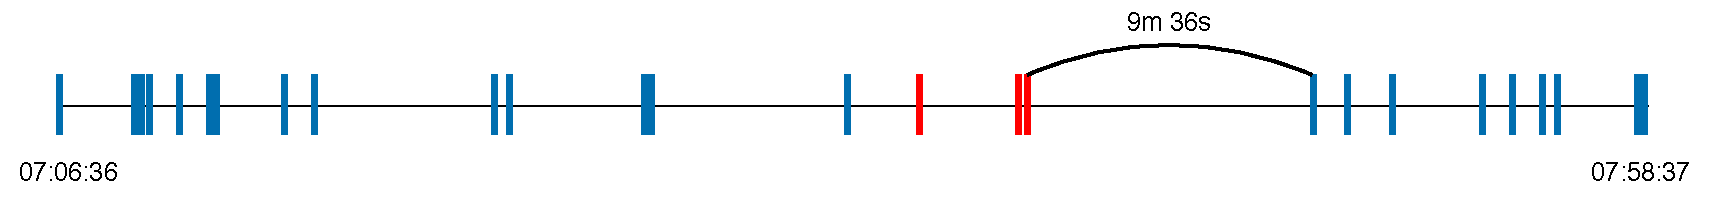
\includegraphics[width=\textwidth]{diagrams/sensor_eval.drawio.pdf}
    \caption{Timeline with sensor readings}
    \label{fig:field_test_sensor_readings}
\end{figure}


\section{Discussion}
\label{sec:eval_discussion}
The performance and cost of the developed system depend mainly on the blockchain used as infrastructure. The selection of such a blockchain thus is of significant importance and must be chosen with great diligence. The current prototype deployed on the sepolia testnet demonstrates the influence of different factors, such as network congestion and priority fees on the time needed for a transaction to be completed. On the testnet, the average response time with a fixed gas price of 30 Gwei is reasonable and could support a real-life scenario. However, this is not representative of the mainnet.

However, the gas consumption of the \gls{sc} functions can be directly adapted to any block-chain running the same \gls{evm} version. The analysis shows that executing a simple scenario on the Ethereum network can be very costly. Polygon presents a solution to this issue as our cost estimation is reduced by a factor of over 422. On Ethereum, the total cost of a scenario is quite costly, but considering the artwork's potential value, we think it could be acceptable for a real-life scenario. With Polygon, the estimated total cost is minimal and acceptable.

The security risks illustrated in Section \ref{sec:security_analysis} prevent the system from being used in a real-life artwork transportation scenario. The developed system serves as a proof of concept, and the security vulnerabilities must be mitigated for a production version.

The intervals of successful readings by the sensor have shown to be inconsistent and leave large gaps between readings. Unfortunately, the quality of the sensor would not be enough to support a real-life use case. A suitable sensor should be able to consistently record at shorter intervals preferably less than a minute long. The reason for the sensor's poor performance is unclear. Possible explanations include a timing issue in the communication between the board and the sensor, voltage fluctuations as the board was powered by a portable power bank or other environmental factors. We believe that this issue could easily be solved by using a higher quality board with integrated sensors such as the B-L462E-CELL1 Discovery kit by ST \cite{stmdevice}. 



\chapter{Summary and Conclusions}
\label{chap:summary}
This chapter aims to conclude the thesis with a summary, conclusions, and potential future work based on the insights gained during development and the limitations of the system.

\section{Summary}
This thesis proposes a novel system to monitor and track artwork during transportation. The system is designed to include both blockchain and \gls{iot} to improve transparency and traceability in the art world. The idea is to attach an \gls{iot} device to the physical artwork that records and stores environmental data critical to the integrity of the artwork. The logging device evaluates the recorded data against a predefined threshold and alerts the stakeholders if any deviations occur. Any data associated with the artwork is stored on the blockchain to serve as an indisputable record of events. To create a proof of concept for this proposed system, a prototype was realized within the scope of this thesis.

The first step was to establish the theoretical background for this project through a literature review. The thesis introduced the concepts of blockchain, \gls{iot}, \glspl{sc}, and continued with a review of related work. The focus was placed on gathering existing solutions or work that use either blockchain, \gls{iot}, or both in tracking and monitoring systems. The results of the literature review were discussed and used as inspiration for the design of the proposed system.

The design of the system includes a description of a simplified artwork tracking scenario that should be supported by the final prototype. The architecture of the system was then derived from this simplified scenario. The final system comprises a frontend user interface, a backend server, a \gls{sc}, and the \gls{iot} device. The frontend is designed to provide a user-friendly interface to the backend server. The backend server exposes a \gls{rest} \gls{api} to interact with the \gls{sc}. The developed \gls{sc} defines the unique digital counterpart of physical artwork as a \gls{nft}. By storing additional details on the \gls{sc}, it becomes feasible to register stakeholders as key actors. Their designated blockchain identities can then be used to access information about the artwork status or request modifications. Authorization is handled by the \gls{sc} itself through a role-based policy while authentication is handled on the server by challenging users to provide proof of ownership. The \gls{iot} device is designed to record temperature and humidity data and report violations of a predefined threshold via the \gls{api} to the \gls{sc}.

The established design and architecture were then implemented in the form of a prototype. The \gls{sc} was implemented in Solidity and deployed to the sepolia testnet. The backend server is written in Python and uses the web3py library to execute contract functions by initiating transactions. Those functions are then exposed as \gls{api} endpoints using the Flask framework. The backend server is deployed to the web as a Google Cloud-run service. The frontend is built using react and provides a \gls{gui} for the \gls{api} endpoints. Using Metamask the user can easily authenticate to the backend server by signing a challenge message and providing proof of ownership over the Ethereum account used. Lastly, to monitor humidity and temperature a Rock Pi was used with a DHT-22 sensor attached. The software for the logger is written in Python. 

The system was evaluated in terms of cost, performance, and security as well as a simulated artwork tracking scenario. The cost analysis was performed on the sepolia testnet and used the recorded gas consumption of function executions to estimate the transaction fees on the mainnet. The analysis also includes an estimation of the fees if the system was deployed on the Polygon network. To evaluate the performance of the system, the requests to the \gls{api} were timed multiple times and the resulting average was discussed. To evaluate the security of the system, several potential threat scenarios were analyzed and rated in terms of security risk.  The field test involved deploying a \gls{sc} instance, minting an \gls{nft}, registering the actors, requesting the artwork to be delivered, approving a status change, reporting a simulated violation, and finally delivering the artwork and changing the status to delivered. The transportation scenario included the logging device being transported outside for roughly an hour. 

\section{Conclusions}
A prototype system to monitor and track artwork using \gls{iot} and blockchain technology was successfully designed, implemented, and evaluated. The general objective has been achieved by this prototype. The system is capable of creating an \gls{nft} as a digital counterpart of artwork. The owner of the artwork is then able to register other stakeholders and effectively give them read/write permissions to information about the artwork and its current status. By attaching a logging device to the artwork, the system can monitor environmental conditions and report any deviations to the system. Those violations are then irrefutably stored on the blockchain. Furthermore, the transaction history on the blockchain can be used to trace ownership and custody of the artwork. The system also provides a user-friendly frontend interface as well as an abstracted \gls{rest} \gls{api} to interact with the system and the underlying \gls{sc}.

The development of the system presented major challenges. For instance, authenticating to the system involves signing a challenge message with a private key. This process can be cumbersome to achieve without proper wallet integration. To overcome this challenge we decided to integrate the popular wallet provider Metamask in our frontend. With this integration, the authentication process is as simple as clicking a button. Another challenge was finding a suitable \gls{iot} device. Initially, the idea was to use a more sophisticated device with integrated sensors. The development on such a board turned out to be more complex and we decided to switch to a simpler device that can run on a familiar operating system like Linux. This choice resulted in a decline in the sensor's quality. Initially, the scope of this thesis also included protecting sensitive data by designing a confidentiality scheme using \gls{zkp}. We decided to leave this for future research as this was intended to be achieved by using existing libraries and frameworks that turned out to be harder to integrate than expected. Instead, we focused on a different set of features for the final prototype.

The developed prototype has been used in a simulated artwork transportation scenario and has been shown to work as intended. Nevertheless, the prototype has some limitations that have to be addressed in future work.

\section{Future Work}
This thesis has demonstrated a minimal prototype to demonstrate a novel approach to artwork tracking and monitoring in transportation scenarios. To arrive at a mature state of the system there is still great room for improvement and further development.

First, it would be essential to upgrade certain components of the system. This may include upgrading to a better sensor as well as adding more sensors to track location, vibration, and other environmental data. With an upgraded \gls{iot} device another field test performed at a larger scale will bring further insight into the feasibility of the system in a real-world scenario.

Secondly, future work should address the security risks outlined in Section \ref{sec:security_analysis}. Primarily the protection of sensitive data should be investigated. This may involve exploring the potential of using \glspl{zkp} to protect data exposed in blockchain transactions \cite{zkdet}.

Lastly, the current design includes a centralized server to provide an interface to the \gls{sc}. This introduces a single point of failure to the system and it might be worth exploring a truly distributed approach. 

\printbibliography
\addcontentsline{toc}{chapter}{Bibliography}


%\begin{thebibliography}{99}
%\addcontentsline{toc}{chapter}{Bibliography}
%
%\bibitem{label} Autoren: Titel, Verlag, \url{http://...}, Datum.

%\end{thebibliography}



% Abbreviations
\setglossarystyle{super}
\printglossary[type=abbreviations, title=Abbreviations]
\markboth{ABBREVIATONS}{}

% Glossary
\renewcommand{\glsnamefont}[1]{\textbf{#1}}
\printglossary[title=Glossary]
\markboth{GLOSSARY}{}

%List of figures and tables
\listoffigures
\addcontentsline{toc}{chapter}{List of Figures}
\listoftables
\addcontentsline{toc}{chapter}{List of Tables}

\appendix

\chapter{Contents of the Repositories}
The system is composed of four repositories that are managed in a GitHub organization. The organization as well as the repositories can be found at:
\begin{center}
    \texttt{\href{https://github.com/orgs/artis-project/repositories}{https://github.com/orgs/artis-project/repositories}}
\end{center}

The implementational details of each component and its associated repository are found in Chapter \ref{chap:implementation}, where each Section is named after the corresponding repository. Additionally, each repository contains a \texttt{README.md} file which contains important information on the component's installation and configuration.

The repository with the name artis-thesis contains the \LaTeX \  source code for this thesis.


\end{document}
